\section{Results}

\subsection{Released cohort and response quality}

The analysis used all 42 participants in the released tables (34 women, 8 men; mean age 23.0 years, SD 4.0, range 19--37). Twenty-one completed each condition order. There were 17{,}114 observed trials of 17{,}136 planned slots: 10{,}068 Audio--Tactile, 5{,}033 Baseline, and 2{,}013 Catch trials. Forty-one sessions were complete; one partial session lacked 22 trials but supplied all 20 Condition $\times$ Phase $\times$ SOA cells. There were 24 Catch false alarms, and no participant exceeded the 30\% Catch exclusion rule. Low-hit-rate flags are reported without adding an exclusion criterion.

Among hit-labelled trials, 105 RTs were missing (80 Audio--Tactile and 25 Baseline). These trials remained in hit-rate denominators. The participant-wide mean $\pm$ 2.5-SD trim removed 382 of 13{,}694 recorded hit RTs, retaining 8{,}916 Audio--Tactile and 4{,}396 Baseline RTs. Adding a 200-ms minimum after trimming removed no further observations. Forty-one participants had the full questionnaire measures and one had PPS measures only.

\subsection{Primary interaction and sensitivity analyses}

Adding the Condition $\times$ Phase $\times$ numeric-SOA term to the trial-level random-intercept ML model did not improve fit, $\chi^{2}(1)=0.024$, $p=.878$. With symmetric Condition/Phase coding and standardized SOA, its estimate was 0.81~ms per SOA SD (SE 5.31; 95\% model-based Wald CI $[-9.60, 11.23]$). This interval permits effects in either direction and does not establish equivalence.

The categorical-SOA comparison gave $\chi^{2}(4)=2.27$, $p=.686$. Excluding the partial session left 41 participants (numeric $p=.807$; categorical $p=.773$). The Control-only Phase $\times$ SOA test was also not detected (numeric $p=.430$; categorical $p=.468$). Allowing a participant random SOA slope yielded $p=.859$. The participant-cell repeated-measures three-way interaction was $F(4,164)=0.99$, Greenhouse--Geisser $\epsilon=0.839$, corrected $p=.406$.

The equal-participant five-SOA slope contrast was 0.03~ms per SOA SD, 95\% CI $[-7.88, 7.95]$, $t(41)=0.008$, $p=.993$. The Monte Carlo sign-flip test used 19{,}999 draws with a fixed seed ($p=.994$). Its exploratory paired JZS factor was $\mathrm{BF}_{10}=0.167$ ($\mathrm{BF}_{01}=6.00$). This normal-likelihood participant model is distinct from the registered mixed model; the slope distribution departed from normality (Shapiro--Wilk $p=.005$).

The exploratory participant-cluster-robust models gave the following three-way terms. Normal Wald intervals use the documented finite-cluster sandwich correction.

\begin{center}
\begin{tabular}{lrrr}
Model & Estimate & 95\% CI & $p$ \\
\hline
Raw RT & -1.543 & $[-9.57, 6.49]$ & $.706$ \\
Log RT & -0.003 & $[-0.01, 0.01]$ & $.614$ \\
Time-on-task-adjusted RT & -1.584 & $[-9.59, 6.42]$ & $.698$ \\
Hit probability (log odds) & 0.001 & $[-0.23, 0.24]$ & $.994$ \\
\end{tabular}
\end{center}

The missing-hit-RT stress tests imputed only the 80 Audio--Tactile hits lacking RTs, then recomputed trimming. Median-only imputation gave $p=.960$; signed $-200$ and $+200$~ms scenarios gave $p=.428$ and $p=.253$, respectively. These specified scenarios do not recover missed-trial RTs or identify the missingness mechanism. Full model coefficients, scaling, diagnostics, intermediate tables, and all stress scenarios are in the companion's downloadable report.

\begin{figure}[htbp]
\centering
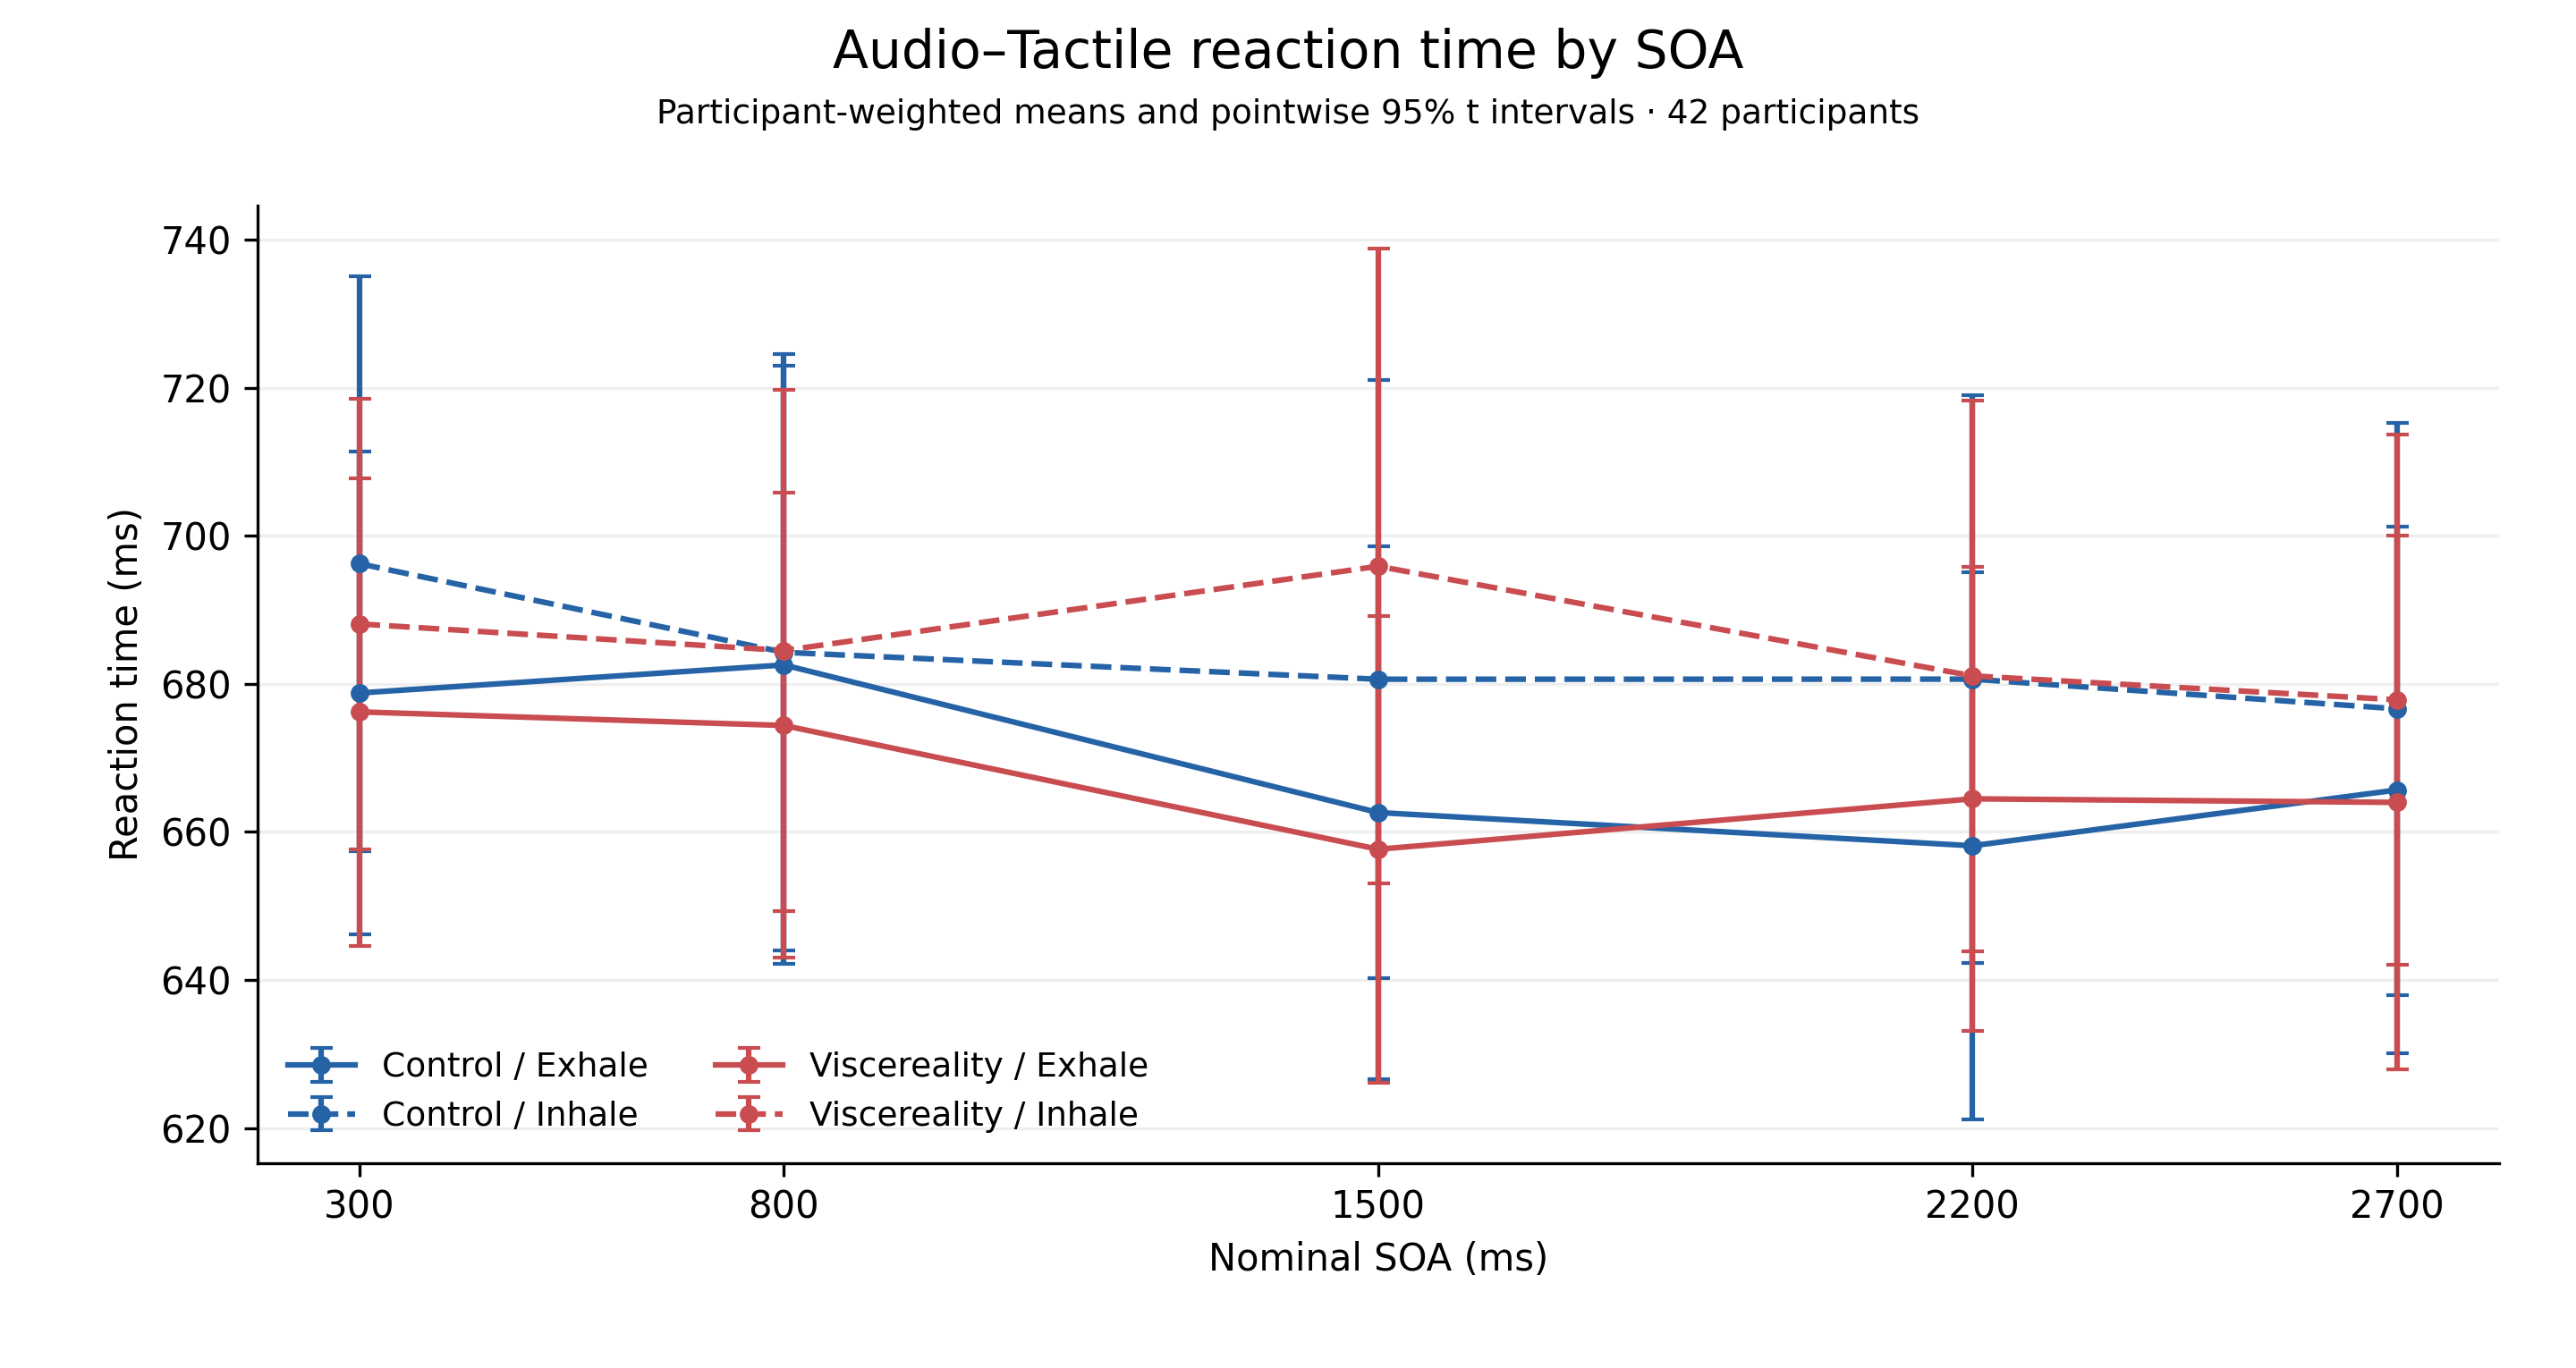
\includegraphics[width=\textwidth]{study5_current_rt_soa_curves.png}
\caption{\textbf{Audio--Tactile RT by SOA, Condition, and instructed respiratory phase in the 42-person cohort.} Each point averages participant means with equal person weight; all cells contain 42 participants. Intervals are pointwise 95\% $t$ intervals across participant means. Longer SOAs correspond to nearer nominal auditory positions. Lines connect means and are not sigmoid fits; inference comes from the stated models.}
\label{study5:fig:current_rt_soa}
\end{figure}

\subsection{Sigmoid viability and descriptive PPS shape}

None of 168 trial-level participant $\times$ Condition $\times$ Phase sigmoid fits reached $R^{2}\geq .70$ (median $R^{2}=0.038$; maximum 0.419). The largest saturated five-SOA trial-level $R^{2}$ ceiling was 0.430. Thus no deterministic sigmoid of these SOAs could reach .70 in any cell, independent of the particular nonlinear optimizer or parameter bounds. Sigmoids improved unpenalized in-sample RMSE over a line in 164/168 cells; this does not establish stable boundaries.

Fitting four parameters to five SOA means instead yielded 79/168 qualifying cells and 3 participants passing all four cells, with none having four bound-free fits. Such fits have one residual degree of freedom and were not used to rescue the failed trial-level gate. Replacing approximate registered distances with trajectory-implied positions left the trial-level pass count at zero. Parameter-bound diagnostics and group fits are supplied descriptively. Participant midpoint/sharpness contrasts and their MAIA-2 or pictographic associations were not estimable under the planned fit gate.

\subsection{Baseline, sound, and order diagnostics}

Across ten supplementary paired contrasts, Holm adjustment was applied as one family. Overall Audio--Tactile minus within-Condition/Phase mean Baseline RT was -18.81~ms, 95\% CI $[-27.00, -10.63]$, unadjusted $p<.001$, Holm $p<.001$. Baseline Inhale minus Exhale RT was 18.08~ms, 95\% CI $[3.28, 32.88]$, unadjusted $p=.018$, Holm $p=.143$. The Baseline Condition $\times$ Phase contrast was 17.43~ms, 95\% CI $[1.56, 33.30]$, unadjusted $p=.032$, Holm $p=.225$. These checks neither establish phase invariance nor provide adjusted evidence of a Baseline phase difference.

The far-minus-near Audio--Tactile difference was 13.80~ms, 95\% CI $[-1.82, 29.42]$; the analogous Baseline nominal-label difference was 11.69~ms, 95\% CI $[-6.90, 30.28]$. Their difference was 2.11~ms, 95\% CI $[-18.44, 22.66]$. Far Audio--Tactile minus Baseline was -10.50~ms using the Condition/Phase reference and -24.83~ms using the same nominal SOA label (Holm $p=.023$ for the latter). Equal labels do not establish cue-time matching; these differences cannot isolate auditory proximity or remove temporal expectancy.

Pink-minus-white Audio--Tactile RT was -2.86~ms, 95\% CI $[-9.30, 3.58]$. Among the 20 participants with all four noise types available, the exploratory Friedman test gave $\chi^{2}(3)=7.80$, $p=.050$. This availability-defined subset cannot be assigned to an acquisition version from the released tables. The two order subgroups each contained 21 participants; their slope contrasts were -4.19~ms, 95\% CI $[-14.64, 6.27]$, and 4.25~ms, 95\% CI $[-8.27, 16.78]$. These descriptive subgroup results do not establish order equivalence.

\begin{figure}[htbp]
\centering
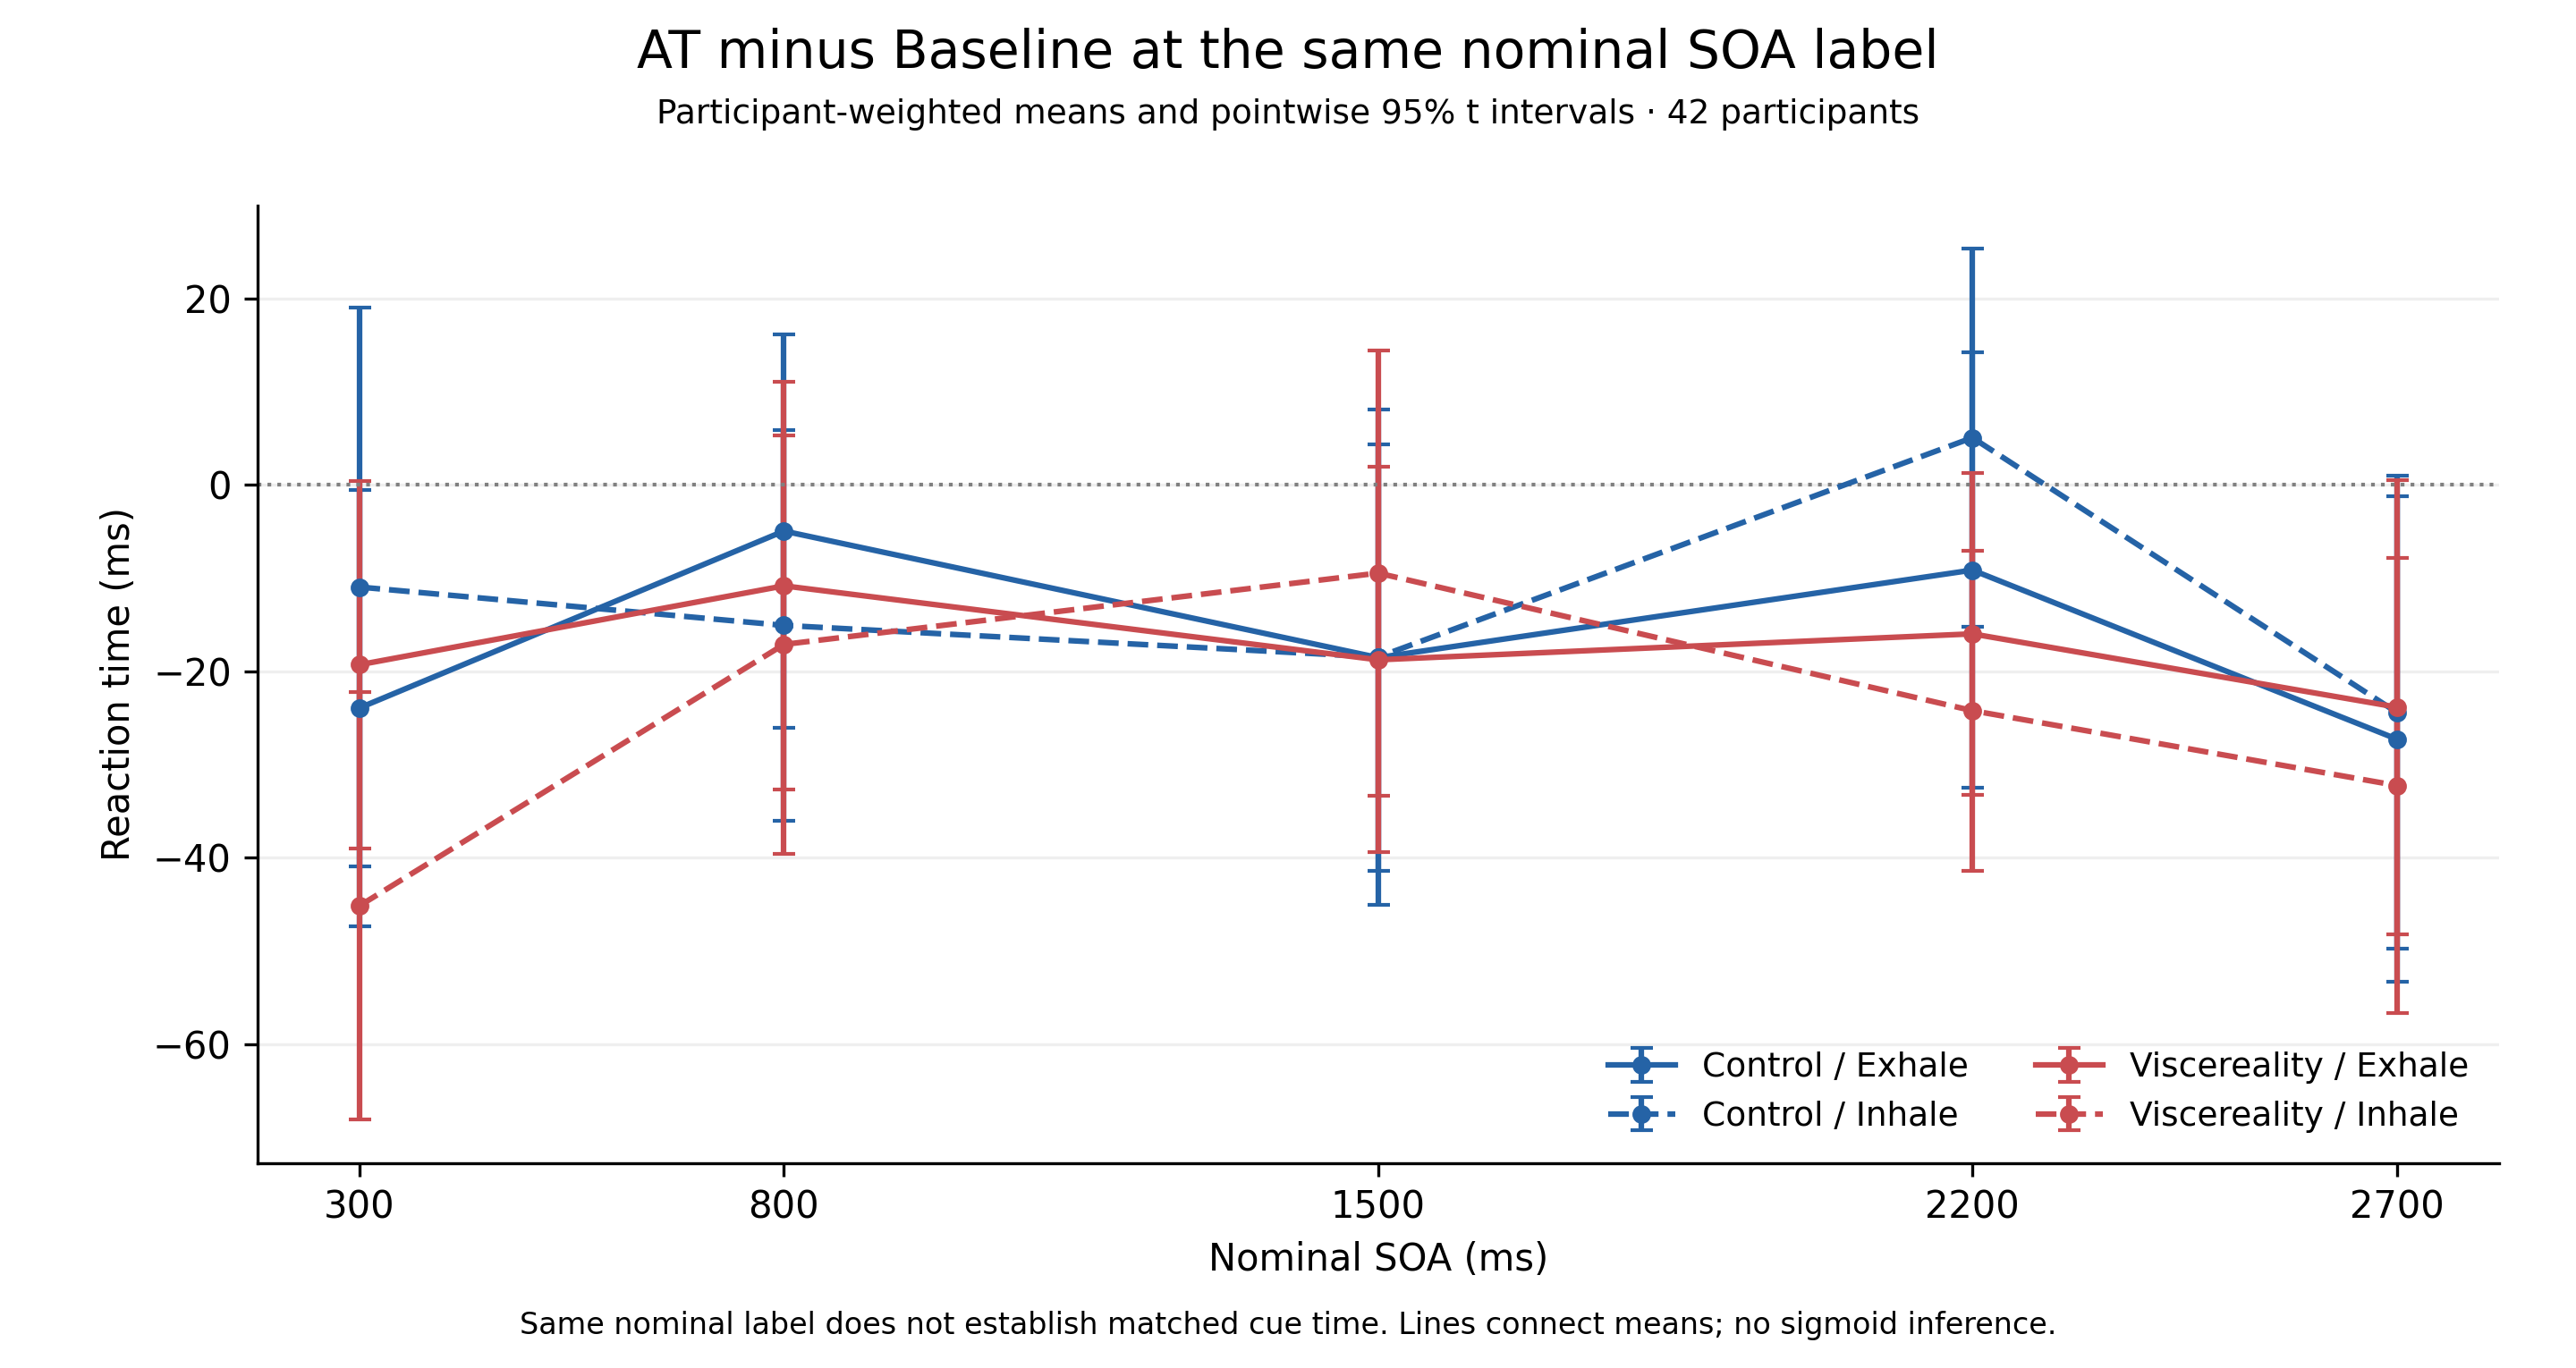
\includegraphics[width=\textwidth]{study5_delay_matched_facilitation.png}
\caption{\textbf{Exploratory Audio--Tactile minus Baseline RT paired by nominal SOA label.} Points average 42 participant differences within Condition $\times$ Phase $\times$ label. Negative values indicate faster Audio--Tactile responses. Baseline has no sound; matching labels does not establish equal trial-relative tactile-cue time. Intervals are pointwise 95\% $t$ intervals across participants. Lines connect means and carry no boundary inference.}
\label{study5:fig:delay_matched_facilitation}
\end{figure}

\subsection{Reproducibility and evidence limits}

All reported behavioral computations were executed in the marimo browser companion with Pyodide, Python 3.14.2, NumPy 2.4.3, SciPy 1.17.1, and Matplotlib 3.10.8. The archived browser download records input, code, and output SHA-256 hashes. Native reference checks independently verified random-intercept ML fits, cluster-robust linear and binomial coefficients/uncertainty, repeated-measures $F$ statistics, and JZS quadrature. A failed or unavailable check is distinguished from a computed null result.

The released CSVs do not contain waveforms, belt recordings, acquisition-version labels, collection dates, or the private provenance needed to identify two historically documented RT-onset variants. The browser analysis therefore does not rerun waveform timing, measured respiratory compliance, pilot-date classification, version-specific contrasts, or that source-definition exclusion. Historical source audits remain historical evidence, rather than new 42-person verification.
